\documentclass{beamer}
\usetheme{default}
\usepackage{booktabs}
\usepackage{graphicx}
\usepackage{subfigure}
\usepackage{caption}
\captionsetup{font=scriptsize}
\graphicspath{ {./figure/}{./figure2/}}

\title{Reinforcement Learning based Decision Tree}
\author{Shangtong Gui\\Advisor: Junfeng Yang, Columbia University}

\begin{document}

\begin{frame}[plain]
    \maketitle
\end{frame}

\begin{frame}{Motivation}
	\begin{block}{Interpretability of Decision Tree}
		Black Box VS Interpretable Tree Structure
	\end{block}
	\begin{block}{Greedy Stragety}
		Only considering immediate information gain at the current splitting node\\
		Sub-optimal
	\end{block}
	\begin{block}{Long Term Vision}
		Search for splitting strategies in the global search space
	\end{block}
\end{frame}

\begin{frame}{Implementation}
	\begin{block}{Action}
		Decide which feature should be splitted.\\
		Feature Vector: $a$\\
		Chosen Feature: $argmax(a)$
	\end{block}
	\begin{block}{Policy Network}
		Policy Network: $F$\\
		Inputs: Node Embedding $x$, Parent's Topology Embedding: $h_p$
		Outputs: Action $a$, Topology Embedding: $h_{true},h_{false}$\\
		$$h_{true},h_{false},a = F(x,\hat{h_p})$$
	\end{block}
\end{frame}

\begin{frame}{Reward BackPropagation}
	
	\begin{block}{Reward}
		Reward under metric $m$: $R_m$, ($m$ could be f1-score, auc, or just accuracy)\\
		Loss function: $\theta$ denotes the policy parameters.\\
		$$J(\theta) = E_{P(a_1:a_T,\theta)[R_m]}$$,
	\end{block}
	 
	\begin{block}{Approximation}
		REINFORCE(Ronald J Williams, 1992) is a policy gradient method.\\
		$$
		\nabla J(\theta) = 
		E_{x\sim P_{data}}\frac 1 L  \sum_{l=1}^L \frac 1 T_l \sum_{t=1}^{T_l} \nabla_\theta log P(a_t^l|a_{t-1}^l;\theta)(R_x - b)
		$$
	\end{block}

	
\end{frame}

\begin{frame}{Experimental Results}
	\begin{block}{Statlog (German Credit Data)}
		\begin{table}[]
			\begin{tabular}{llll}
				\hline
				& auc    & acc    & f1     \\ \hline
				Baseline & 0.6805 & 0.7200 & 0.7077 \\
				RLTree   & 0.7544 & 0.7400 & 0.7080 \\ \hline
			\end{tabular}
		\end{table}
	\end{block}
	\begin{figure}{}
		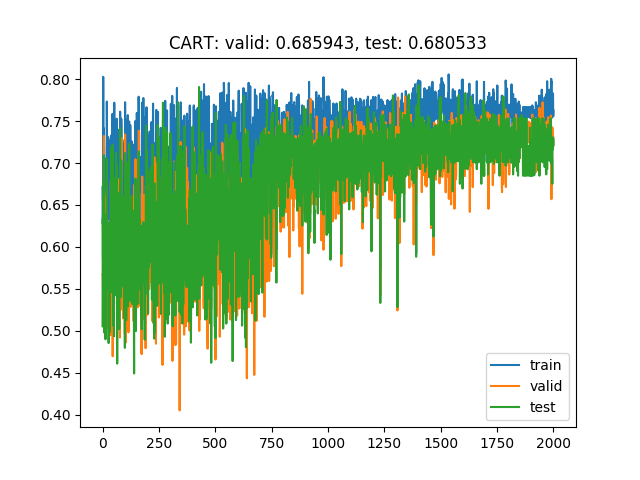
\includegraphics[scale=0.4]{german_auc_sample_curve}
		\caption{AUC metric}
	\end{figure}
\end{frame}

\begin{frame}{Experimental Results}
	\begin{block}{Home Credit Default Risk Dataset}
	\begin{table}[]
		\begin{tabular}{llll}
			\hline
			& auc    & acc    & f1     \\ \hline
			Baseline & 0.6689 & 0.9216 & 0.8840 \\
			RLTree   & 0.6657 & 0.9163 & 0.8763 \\ \hline
		\end{tabular}
	\end{table}
	\end{block}
	\begin{figure}{}
		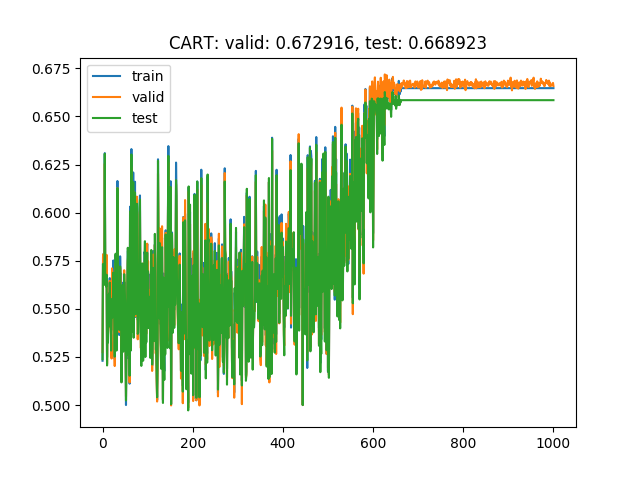
\includegraphics[scale=0.4]{credit_auc_sample_curve}
		\caption{AUC metric}
	\end{figure}
\end{frame}

\begin{frame}{Experimental Results}
	\begin{block}{Breast Cancer}
		\begin{table}[]
			\begin{tabular}{llll}
				\hline
				& auc    & acc    & f1     \\ \hline
				Baseline & 0.9514 & 0.9216 & 0.9363 \\
				RLTree   & 0.9615 & 0.9160 & 0.9089 \\ \hline
			\end{tabular}
		\end{table}
	\end{block}
	\begin{figure}{}
		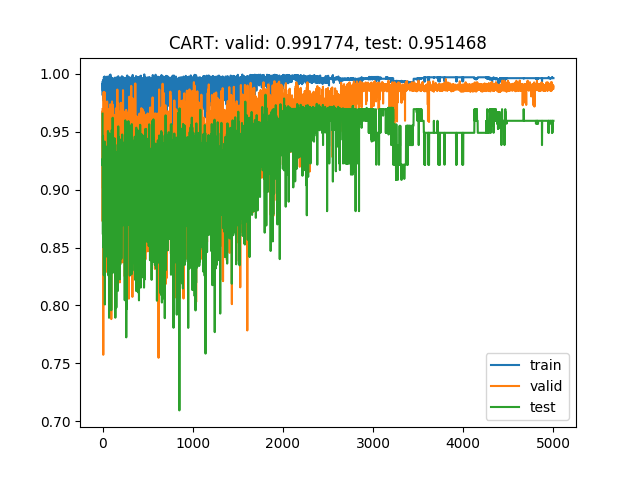
\includegraphics[scale=0.4]{breast_cancer_auc_sample_curve}
		\caption{AUC metric}
	\end{figure}
\end{frame}



\begin{frame}{Experimental Results}
	\begin{block}{Pima Indians Diabetes Database}
		\begin{table}[]
			\begin{tabular}{llll}
				\hline
				& auc    & acc    & f1     \\ \hline
				Baseline & 0.7909 & 0.7395 & 0.7315 \\
				RLTree   & 0.7846 & 0.7395 & 0.7618 \\ \hline
			\end{tabular}
		\end{table}
	\end{block}
	\begin{figure}{}
		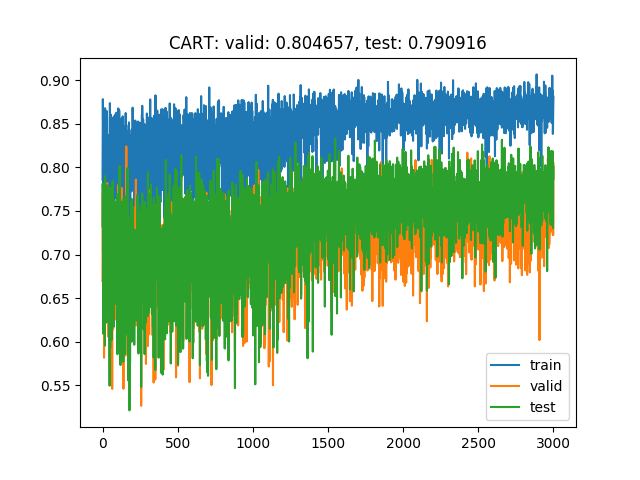
\includegraphics[scale=0.4]{pima_auc_sample_curve}
		\caption{AUC metric}
	\end{figure}
\end{frame}

\begin{frame}{Experimental Results}
	\begin{block}{Heart Disease}
		\begin{table}[]
			\begin{tabular}{llll}
				\hline
				& auc    & acc    & f1     \\ \hline
				Baseline & 0.8241 & 0.8382 & 0.8384 \\
				RLTree   & 0.8692 & 0.7941 & 0.8241 \\ \hline
			\end{tabular}
		\end{table}
	\end{block}
	\begin{figure}{}
		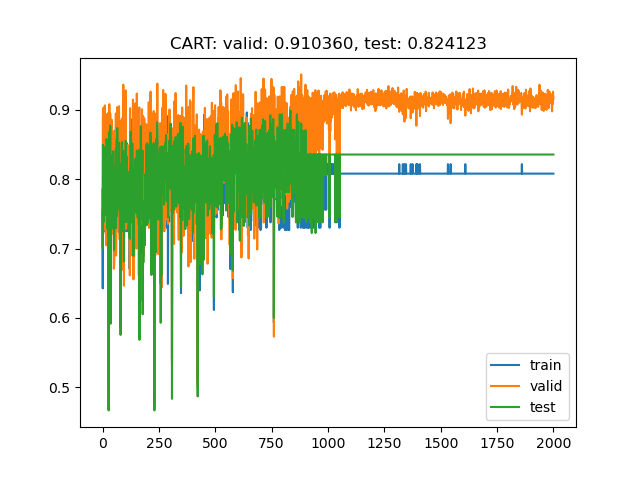
\includegraphics[scale=0.4]{heart_auc_sample_curve}
		\caption{AUC metric}
	\end{figure}
\end{frame}


\begin{frame}{Future Work}
	\begin{block}{Embdedding Method}
		Embedding Action\\
		Embedding Tree
	\end{block}
	\begin{block}{Ensemable Decision Tree}
		Multi-agent problem
	\end{block}
\end{frame}

\begin{frame}[plain,c]
	%\frametitle{A first slide}
	
	\begin{center}
		\Huge Thanks
	\end{center}
	\begin{center}
		Q\&A
	\end{center}
	
\end{frame}

\end{document}
